\section{Cubic Mechanism}
  In this section, we present two mechanisms to calculate the sending rates of 
  the packets of the p-stream. One mechanism is the ideal cubic mechanism one 
  would like to use. However, because the equations involved are difficult to 
  solve in the kernel, we present another mechanism that is more suitable for 
  kernel implementation but not as accurate as the ideal mechanism.

  \subsection{Ideal Cubic Mechanism}
    To generate finer granularity close to the average sending rate of the 
    p-stream $r_{avg}$ and coarser granularity far from it, a cubic function 
    comes to mind. The mechanism presented below consists of a cubic function 
    of the index $i$ of the packets in the p-stream. The ideal cubic mechanism 
    consists of the following expressions:
    \begin{IEEEeqnarray}{rCl}
      r_0 & = & \frac{r_{avg}}{m} \label{value0} \\
      r_i & = & C(i - K)^3 + r_{avg} \label{rvalue}
    \end{IEEEeqnarray}
    where $m$ is a parameter that determines the range of rates probed. Using 
    the value of $r_0$ given in equation \eqref{value0} and equation 
    \eqref{rvalue} we can calculate the value of $K$ as follows.
    \begin{IEEEeqnarray}{rCl}
      r_0 & = & C(0 - K)^3 + r_{avg} \\
      \frac{r_{avg}}{m} & = & -CK^3 + r_{avg}
    \end{IEEEeqnarray}
    This gives
    \begin{equation}
      K = \sqrt[3]{\frac{r_{avg}}{C} \left (1 - \frac{1}{m} \right )}
    \end{equation}
    Also, C has a value that satisfies
    \begin{IEEEeqnarray}{rCl}
      r_{avg} & = & \frac{N}{\frac{1}{r_0} + \frac{1}{r_1} + \ldots + 
      \frac{1}{r_{N-1}}} \\
      r_{avg} & = & \frac{N}{\frac{m}{r_{avg}} + \frac{1}{C(1-K)^3 + r_{avg}} +
      \ldots + \frac{1}{C(N - 1 - K)^3 + r_{avg}}}
    \end{IEEEeqnarray}

    Unfortunately, there is no closed form solution for the above equation. In 
    fact, using Mathematica assigning values to $m$, $r_{avg}$, and $N$ and 
    trying to solve the equation also does not give a solution.

  \subsection{Cubic Mechanism Used}
    Since the mechanism described in the previous section can not be used as 
    the mechanism to compute the sending rates of the packets in the p-stream, 
    we present another mechanism that can actually be implemented in the 
    kernel. This mechanism looks at the sending rate during the p-stream as a 
    function of time rather than as a function of the index of the packets in 
    the p-stream. Suppose $N$ is the number of packets in the p-stream and $P$ 
    is size of the packets. Then, the duration of the p-stream is
    \begin{equation}
      L = \frac{N*P}{r_{avg}}
    \end{equation}
    Since we want the rates of the packets of the p-stream to follow a cubic 
    curve, we define a cubic function with its plateau at $r_{avg}$.
    \begin{equation}
      r(t) = C \left (t - \frac{L}{2} \right )^3 + r_{avg}
    \end{equation}
    We impose the condition that $r(0) = \frac{r_{avg}}{m}$. Using this 
    condition and the above equation we can solve for C.
    \begin{equation}
      C = \frac{8}{L^3} \left (1 - \frac{1}{m} \right ) r_{avg}
    \end{equation}
    Thus, $r(t)$ becomes
    \begin{equation}
      r(t) = \frac{8}{L^3} \left (1 - \frac{1}{m} \right )r_{avg} \left 
      (t - \frac{L}{2} \right )^3 + r_{avg} \label{cubic}
    \end{equation}

    If we integrate $r(t)$ from $t = 0$ to $t = L$ we get exactly $N \cdot P$ 
    as the result. Thus if TCP Rapid exactly has a sending rate given by 
    $r(t)$ during the duration of the p-stream, the p-stream will have an 
    average rate of $r_{avg}$. However, the p-stream has a finite number of 
    packets and the entire packet will be sent at a single rate. We use $r(t)$ 
    to set the rate of the packets of the p-stream as follows.
    \begin{IEEEeqnarray}{rCl}
      r_0 & = & \frac{r_{avg}}{m} \\
      r_i & = & r \left ( \sum_{k = 0}^{i-1} \frac{P}{r_k} \right ) 
      \text{ for } 1 \le i \le N - 1
    \end{IEEEeqnarray}
    where the $i^{th}$ packet is sent at time
    \begin{equation}
      \sum_{k=0}^{i-1} \frac{P}{r_k}
    \end{equation}
    from the beginning of the p-stream. 
    
    Figure \ref{mechanism} shows a plot of 
    equation \eqref{cubic} for the values of $N = 15$, $P = 1040$ bytes, 
    $m = 2$, and $r_{avg} = 400$ Mbps. The width of each colored rectangle 
    represents the time it takes to transmit the corresponding packet while
    the height represents the rate at which the corresponding packet is sent. 
    The horizontal line in Figure \ref{mechanism} represents the value of 
    $r_{avg}$ while the vertical red line at the far right represents the 
    value of $L$, the duration of the p-stream. However, we can see from 
    Figure \ref{mechanism} that to transmit the last packet of the p-stream 
    (blue colored rectangle on the far right), we need more time than $L$ 
    seconds since the blue rectangle goes beyond the red line. This, shows 
    that the average rate of the p-stream will not be exactly $r_{avg}$, but 
    less than $r_{avg}$. In fact, for the values of $N = 15$, $P = 1040$ 
    bytes, $m = 2$, and $r_{avg} = 400$, the harmonic mean of the packet rates
    obtained with this mechanism is $388.468$ Mbps which is smaller than 
    $r_{avg} = 400$ Mbps.
    \begin{figure}[hbp]
      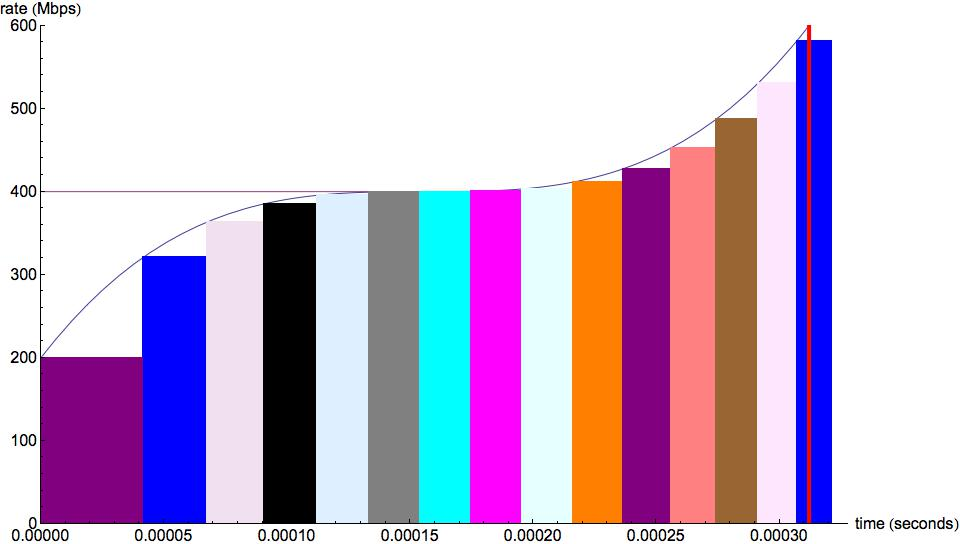
\includegraphics[scale=0.4]{img/cubic.jpg}
      \caption{The cubic mechanism used}
      \label{mechanism}
    \end{figure}

    Figure \ref{rates} plots the sending rates of the packets versus their 
    index in the p-stream. We notice that we have a finer granularity close to 
    the value of $r_{avg}$. This means that the mechanism is better suited 
    when the new available bandwidth is close to the previous available 
    bandwidth estimate.
    \begin{figure}[h]
      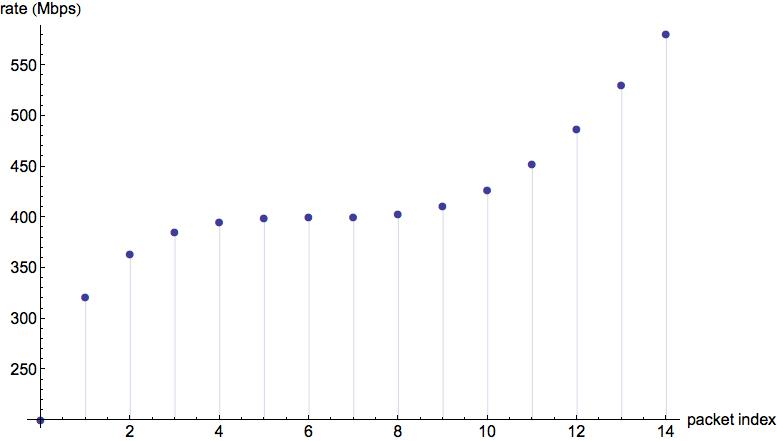
\includegraphics[scale=0.45]{img/rates.jpg}
      \caption{The sending rates of the packets in the p-stream}
      \label{rates}
    \end{figure}
